%!TEX program = pdflatex
% Full chain: pdflatex -> bibtex -> pdflatex -> pdflatex
\documentclass[lang=en,12pt]{elegantpaper}
\usepackage{url}


\title{Gomoku Project Report}
\author{WU Yechang}
\institute{11711918}
\date{\today}

\begin{document}

\maketitle

\begin{abstract}
Gomoku, also called Five in a Row, is an abstract strategy board game.
It is traditionally played with Go pieces (black and white stones) on a Go board, using 15$\times$15 of the 19$\times$19 grid intersections.
The game is known in several countries under different names.While playing Gomoku, players alternate turns placing a stone of their color on an empty intersection. The winner is the first player to form an unbroken chain of five stones horizontally, vertically, or diagonally.

This report includes my experience in making a Gomoku AI from zero. Relative code can be found on \href{https://github.com/Wycers/GomokuAI}{https://github.com/Wycers/GomokuAI}
\keywords{Gomoku, Game AI, Search Tree}
\end{abstract}


\section{Preliminaries}
\subsection{Problem Description}
In SUSTech CSE CS303 course, students are required to submit a Gomoku AI program to an online platform to battle with other Gomoku programs and get ranked.
On this battle platfrom, there are some limitations:
\begin{itemize}
  \item Students' program is ought to be one single python file.
  \item The python file size is limited to a maximum of 10MB.
  \item Machine learning framwork such as tensorflow, pytorch, etc. is disallowed. But Numpy is allowed.
  \item A program can only take up to 5 seconds to make a move and can only use 180 seconds in one game.
  \item A program can only uses up to 100MB of memory.
\end{itemize}

\subsection{Software}
This project is written in \textsl{Python} with editor \textsl{Visual Studio Code}.
The main testing platform is Windows 10 Professional Edition (version 1903) with Intel$^\circledR$ Core$^{\text{TM}}$ i7-8700 @ 3.20GHz with 6 cores and 12 threads.
\subsection{Problem Applications}
\begin{itemize}
  \item Exercise python programming skills
  \item Implement search algorithm
  \item Learn how general game AI works
\end{itemize}

\section{Methodology}
\subsection{Notation}
\begin{itemize}
  \item {\bf Color}:
  \item {\bf Evaluation of chessboard}: A score representing the index of pros and cons of chessboard for current player.
  Generally, if the valuation of chessboard is higher, my program will more likely to win.
  \item {\bf Evaluation of position}: A score representing the the index of pros and cons of chessboard position for current player.
  Generally, if the valuation of position is higher, my program will more likely to make a move at this position.
\end{itemize}

\subsection{Date Structure}

\begin{itemize}
\item {\bf Stage}: A 2d-array representing status of chessboard.
Assume that a Stage $s$ is used to represent a chessboard $C$, and

if $C$ has a {\bf BLACK} chess at row $i$, column $j$, $s[i][j] = -1$;

if $C$ has a {\bf WHITE} chess at row $i$, column $j$, $s[i][j] = 1$;

if $C$ is {\bf empty} at row $i$, column $j$, $s[i][j] = 0$.

\item {\bf Chess pattern}: A 1d-array representing continuous 7 chesses with only one color and empty. For example, 'BEBBBEB' goes to '[-1, 0, -1, -1, -1, 0, -1]' and 'BEBWBEB' is not a chess pattern.
\end{itemize}
\subsection{Model Design}
The problem is that, with input of chessboard and color, ouptut a position where program thinks better.
There is no absolute right moves and wrong moves, but only good moves and bad moves. Here are some solution I have tried.
\begin{itemize}
  \item {\bf Single Step Search}: At each step, use evaluation of position, choose the highest position to make next step;
  if there are many positions has same highest evaluation, choose one of them randomly.
  \item {\bf Minimax Search}: Consider that there are two players are playing Gomoku, when player A is making a move,
  he wants to make his evaluation of chessboard as large as possible.
  But after he making this move, his opponent,
  player B will try to make a move to lower A's evaluation of chessboard. In short, when dealing with gains, it is referred to as "maximin"—to maximize the minimum gain. \cite{minimax}
  So using minimax algorithm to search best evaluation of chessboard after more steps can archive more posibility to win.
  \item {\bf Alpha-Beta}: Alpha–beta pruning is a search algorithm that seeks to decrease the number of nodes that are evaluated by the minimax algorithm in its search tree. It stops evaluating a move when at least one possibility has been found that proves the move to be worse than a previously examined move. Such moves need not be evaluated further. When applied to a standard minimax tree, it returns the same move as minimax would, but prunes away branches that cannot possibly influence the final decision.\cite{alphabeta}
  By using alpha-beta algorithm, program can search more deeper(twice, theoretically).
  \item {\bf AlphaZero}:  The AlphaZero engaged in reinforcement learning, playing against itself until it could anticipate its own moves and how those moves would affect the game's outcome.
  \cite{alphazero} AlphaZero will see players move as input,
  use model pretrained by MCTS search,
  output posibility to win at each position.
  It well played but I give up it because tensorflow is disallowed on platform.
\end{itemize}

\newpage
\subsection{Detail of Algorithm}

\begin{itemize}
  \item {\bf Single Step Search}:
    Evaluate a score for every position and choose the best one.
    \begin{lstlisting}
# input: chessboard, color. output: (x, y) represents my move
pos = (7, 7)  # initial pos: (7, 7) is the center of 15x15 chessboard
mx = 0        # initial mx is 0
for each position in chessboard:
    for all directions:
        pattern = continous 7 chesses in current direction
        tmp = evaluate(pattern)  # use preset parameters to evaluate this pattern
        if tmp > mx:
            mx = tmp
            pos = current position
return pos
    \end{lstlisting}
  \item {\bf Minimax Search}:
    \begin{lstlisting}

search(chessboard, color, depth):
    if depth reaches preset stopping depth:
        return evaluate(chessboard)
    Comparator, Res = min or max, infinity or -infinity
    # if color == self.color, use max and -infinity
    # if color != self.color, use min and infinity
    for all legal position:
        chessboard[position] = color
        tmp = search(chessboard, -color, depth + 1)
        Res = Comparator(Res, tmp)
        # according current player's rule to make a better decision
        chessboard[position] = COLOR_NONE
    return Res

search(chessboard, max)

    \end{lstlisting}

\newpage
  \item {\bf AlphaBeta}:
    \begin{lstlisting}

search(chessboard, color, depth, peer):
    if depth reaches preset stopping depth:
        return evaluate(chessboard)
    Comparator, Res = min or max, infinity or -infinity
    # if color == self.color, use max and -infinity
    # if color != self.color, use min and infinity
    for all legal position:
        chessboard[position] = color
        tmp = search(chessboard, -color, depth + 1)
        Res = Comparator(Res, tmp)
        if Comparator(tmp, peer) == tmp: % At this layer, player will choose peer to tmp
            return Res                   % Cut this branch
        # according current player's rule to make a better decision
        chessboard[position] = COLOR_NONE
    return Res

search(chessboard, max)

    \end{lstlisting}
  \item {\bf AlphaZero}: The AlphaZero engaged in reinforcement learning, playing against itself until it could anticipate its own moves and how those moves would affect the game's outcome.
  \cite{alphazero} AlphaZero will see players move as input,
  use model pretrained by MCTS search,
  output posibility to win at each position.
  It well played but I give up it because tensorflow is disallowed on platform.
\end{itemize}



\section{Empirical Verification}
\subsection{Dataset}
\begin{figure}[ht]
	\centering
	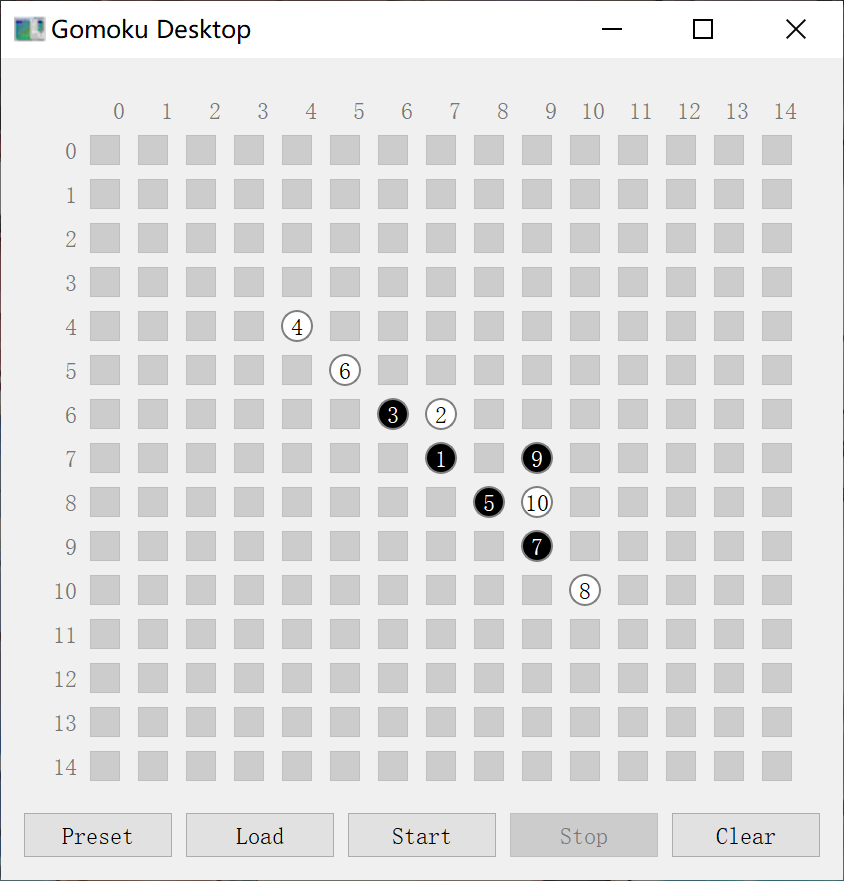
\includegraphics[width=0.6\textwidth]{figure/tool.png}
	\caption{Gomoku Debugger Tool By Ziqin \label{fig:tool}}
\end{figure}
Based on a tool developed by WANG Ziqin, I developed "load" function to quickly generate chessboard from chessboard.log what can be downloaded from Gomoku platform.
The tool also supports AI vs player.
With this tool, I can easily watch running status of my program whiling debugging.
\begin{itemize}
  \item In the usability,
  besides the test cases that the code\_test.py provided,
  I construct some tricky chessboard to test my program's functionality.
  For example, I used some situations that my program is ought to lose after 3 steps to test whether it has long-term consideration.
  \item In the point race, I mainly used chessboard data generated from playing with other players allocated by platform to imporve my program.
  If my program lost in one game, I would download the log file and check which steps my program made is in blame.
  Then adjust the code to let it make a better step in same situation.
  \item In round robin, after the man-machine battle and playto functions are banned,
  I mainly adjust my current program by watching it battling with my older versions and finding the bad step my program made.
\end{itemize}

\subsection{Performance}
My program passed the usability test.
Whiling chessing, my program will use alpha-beta algorithm, pruning among $\frac{1}{4}$ branches, searching 5 layers in depth and highest 5 points at each layer in width.
The average cost time for a single going is around $4-5\text{s}$.
The final rank of my program is {\bf 61 / 200}.


\subsection{Hyper-parameter}
My program has one hyper-parameter \textsl{T}, which is a float number between $0$ and $1$, which is used to adjust the aggressiveness of program.
The opponent pattern score will be multiplied by the param \textsl{T} before being accumulated into evaluation results,
thus the larger the \textsl{T} is, program will consider opponent would make more aggressive moves and take more conservative move for itself.

The rest 128 parameters are used to evaluate the chess pattern.
The 5 in a row pattern has a highest score. The score has adjusted so that sum of several weak patterns would not be greater than a strong pattern.
\subsection{Experimental results}
\begin{itemize}
  \item Pass all the test cases (25) in usability test.
  \item Got rank \#61 in the points race. (Score 86)
  \item Got rank around \#51 in the round robin. (Score 89)
\end{itemize}

\subsection{Conclusion}
Like what I posted on my qzone, Gomoku AI Program is full of fun!
In this lab, I implemented Gomoku AI Program in four versions(basic search, min-max, alpha-beta, alphazero).
My final program can search 5 layers in depth and 5 points in width. The only regret is that I haven't concentrate to adjust one version, leading to a not very outstanding final score. Another obvious issue is that, my program cannot reuse evaluation information calculated before. So my program makes a lot repeating work to evaluate chessboard, which speeds a lot of time. With these issues in mind, if there is an opportunity to improve my program in the future, I will implement incremental updates to make evaluation function able to reuse information before.

During this lab, I tried my best to review many related projects and really learned a lot of things from heuristic search to machine learning, feeling enriched and happy.


\nocite{*}
\bibliography{wpref}

\end{document}
